\section*{Introduction}

\begin{frame}{Introduction}
    \begin{enumerate}
        \item Introduction
    \end{enumerate}
\end{frame}

\begin{frame}{iGem: International Genetically Engineered Machine}
    \begin{figure}
        \centering
        
\includegraphics[width=0.2\textwidth]{images/igem.png}
        \caption{Logo}
        \label{fig:my_label}
    \end{figure}
    iGEM is a synthetic biology competition that gathers the young minds from around the world to collaborate, innovate and tackle complex challenges in the field of biotechnology.
    
    \bigskip

    iGem empowers teams of undergradudate and graduate students to design, build and test novel biological systems and applications.
    
\end{frame}

\begin{frame}{iGem: Software and AI}
    An iGem competition track dedicated to projects based on computational methods.
    \begin{figure}
        \centering
        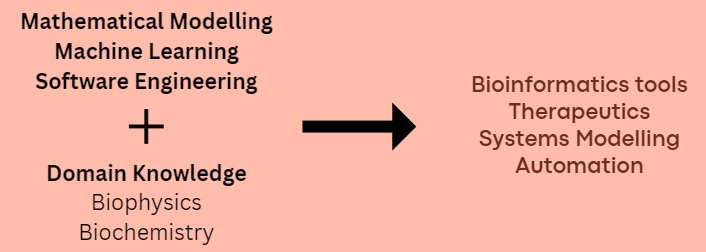
\includegraphics[width=0.8\textwidth]{images/iGemSAI.png}
        \caption{Logo}
        \label{fig:my_label}
    \end{figure}
\end{frame}

\begin{frame}{Computational Biology}

    \begin{figure}
        \centering
        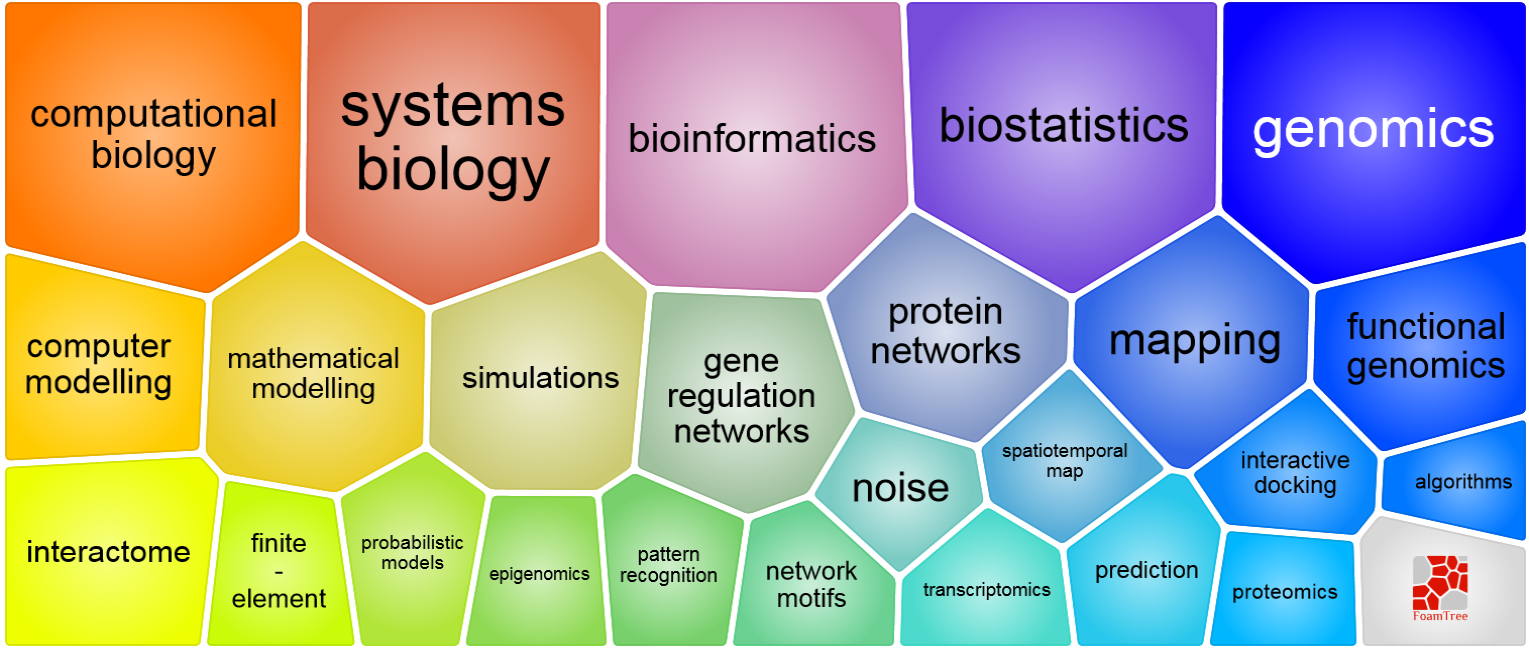
\includegraphics[width=0.8\textwidth]{images/bioinf.png}
        \caption{Comp Bio}
    \end{figure}

    Computational biology refers to the use of data analysis, mathematical modeling and computational simulations to understand biological systems and relationships.


\end{frame}

\begin{frame}{Integrated Modelling of Protein Complexes}
    \begin{figure}
        \centering
        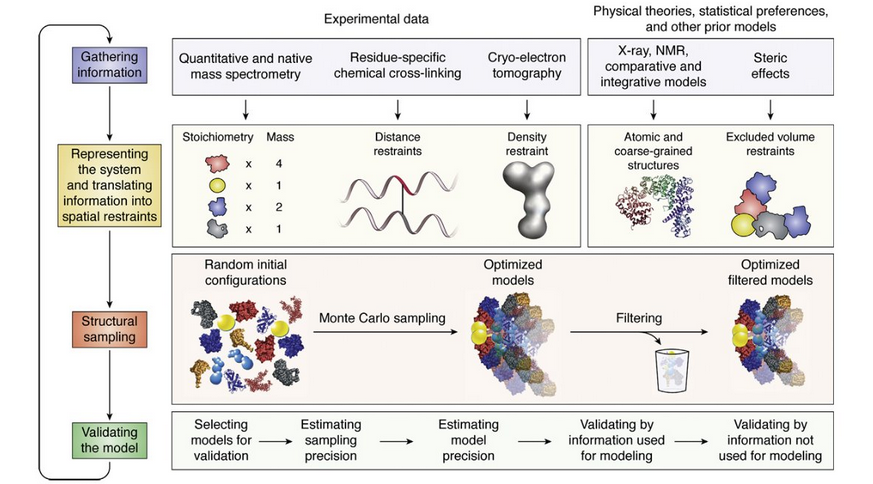
\includegraphics[width=1\textwidth]{images/imp.png}
        \caption{Flowchart representing the IMP}
        \label{fig:my_label}
    \end{figure}
\end{frame}

\begin{frame}
    \begin{figure}[h]
        \centering
        \begin{subfigure}[b]{0.3\textwidth}
            \centering
            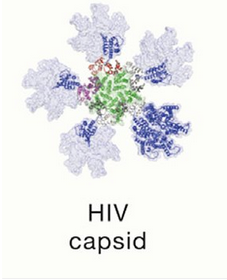
\includegraphics[width=\textwidth]{images/one.png}
            \caption{Deshmukh et al., 2013}
            \label{fig:image1}
        \end{subfigure}
        \hfill
        \begin{subfigure}[b]{0.3\textwidth}
            \centering
            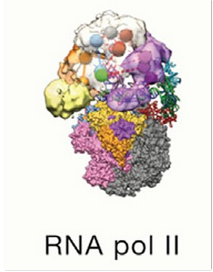
\includegraphics[width=\textwidth]{images/two.png}
            \caption{Murakami et al., 2013}
            \label{fig:image2}
        \end{subfigure}
        \hfill
        \begin{subfigure}[b]{0.3\textwidth}
            \centering
            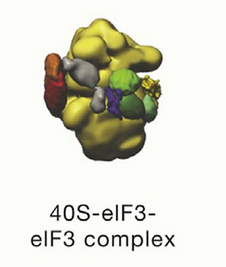
\includegraphics[width=\textwidth]{images/three.png}
            \caption{Erzberger et al., 2014}
            \label{fig:image3}
        \end{subfigure}
        
        \label{fig:three_images}
    \end{figure}
\end{frame}

\begin{frame}{Why Integrated Modelling}
    \begin{enumerate}
        \item Using new information
        \item Maximizing accuracy, precision and completeness
        \item Planning experiments
    \end{enumerate}
\end{frame}

\begin{frame}{Present Landscape}
    \begin{figure}[h]
        \centering
        \begin{subfigure}[b]{0.3\textwidth}
            \centering
            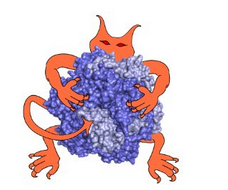
\includegraphics[width=\textwidth]{images/monster.png}
            \caption{IMP,the integrative modelling platform}
            \label{fig:image1}
        \end{subfigure}
        \hfill
        \begin{subfigure}[b]{0.3\textwidth}
            \centering
            
\includegraphics[width=\textwidth]{images/rosseta.png}
            \caption{rosetta}
            \label{fig:image2}
        \end{subfigure}
        \hfill
        \begin{subfigure}[b]{0.7\textwidth}
            \centering
            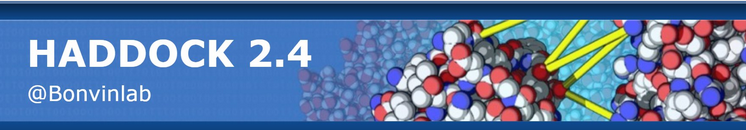
\includegraphics[width=\textwidth]{images/haddock.png}
            \caption{haddock}
            \label{fig:image2}
        \end{subfigure}
    \end{figure}

    
\end{frame}

\begin{frame}

    \begin{figure}
        \centering
        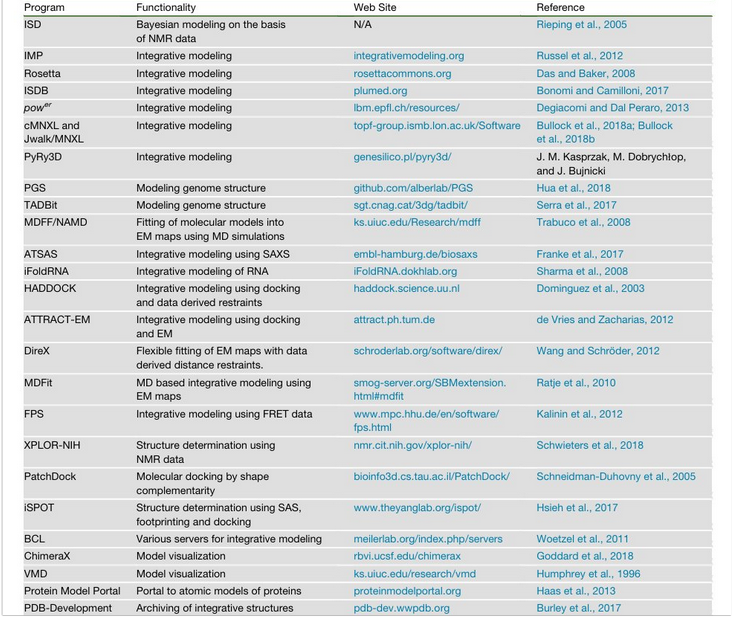
\includegraphics[width=0.8\textwidth]{images/table.png}
        \caption{}
        \label{fig:my_label}
    \end{figure}
    
\end{frame}

\begin{frame}{Our Improvement}
    \begin{figure}
        \centering
        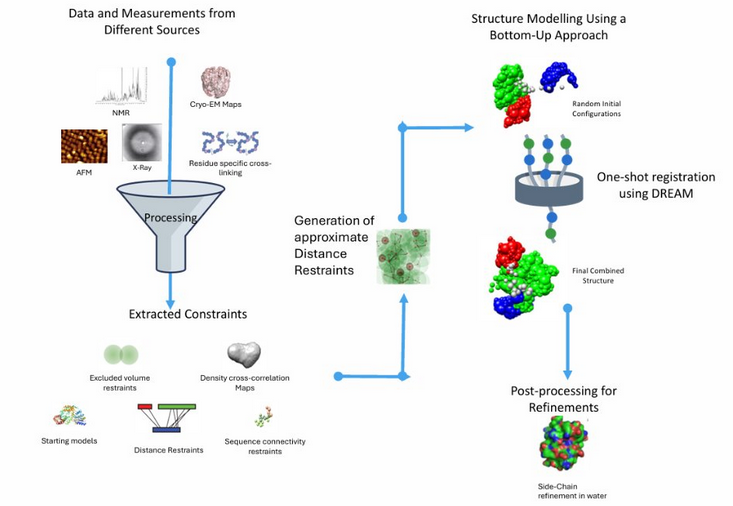
\includegraphics[width=0.7\textwidth]{images/dream.png}
        \caption{Flow Chart}
        \label{fig:my_label}
    \end{figure}

    \begin{enumerate}
        \item Single Shot Registration
        \item Scalability
    \end{enumerate}
\end{frame}
